\section{Limits of Functions}
\label{sec:limits}

\subsection{Limits}
In Section \ref{sec:tangents}, we saw that as the interval over which we calculated got smaller, the secant slopes approached the tangent slope. The {\bf limit}\index{Limit} gives us better language with which to discuss the idea of ``approaches.''
\begin{wrapfigure}{R}{0.25\textwidth}
  \vspace{-20pt}
  \centering
    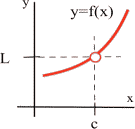
\includegraphics[width=0.24\textwidth]{img/chap2/image011.png} 
\caption{The limit of $f(x)$ as $x\to c$ is $L$.}
\label{fig:2-4-limits}
\vspace{-20pt}
\end{wrapfigure}
The limit of a function describes the behavior (i.e., output) of the function when the variable is near, but not necessarily equal to, a specified number. (See Figure \ref{fig:2-4-limits}.)

\begin{definition}[Limit]
If the values of $f(x)$ get closer and closer, as close as we want, to one single number $L$, as we take values of $x$ very close to (but not equal to) a number $c$, then we say, ``the {\bf limit} of $f(x)$ as $x$ approaches $c$ is $L$'' and we write
$$\lim_{x\to c}f(x)=L \enspace .$$
The symbol ``$\to$'' means ``approaches'' or, less formally, ``gets very close to.''
\end{definition}
This definition of the limit isn't stated as formally as it could be, but it is sufficient for our purposes in this textbook.

{\bf Note:}
    \begin{itemize}[label={}]
    \item $f(c)$ is a single number that describes the behavior (value) of $f(x)$ at the point $x=c$.
    \item $\displaystyle\lim_{x\to c}f(x)$ is a single number that describes the behavior of $f(x)$ near, but NOT at, the point $x=c$.
    \item If we have a graph of $f(x)$ near $x = c$, then it is usually easy to determine $\displaystyle\lim_{x\to c}f(x)$.
    \end{itemize}

\begin{example}
Use the graph of $y=f(x)$ in Figure \ref{fig:2-4-limit-ex} to determine the following limits.
\begin{figure}[!ht]
    \centering
    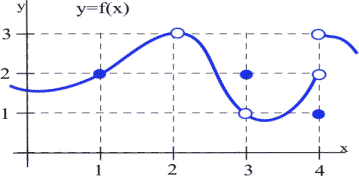
\includegraphics[width=0.4\textwidth]{img/chap2/image012.png}
    \caption{$y=f(x)$}
    \label{fig:2-4-limit-ex}
\end{figure}

\begin{enumerate}[label=(\alph*)]
  \item $\displaystyle\lim_{x\to 1}f(x)$

  \begin{solution}
When $x$ is very close to 1, the values of $f(x)$ are very close to $y=2$. In this example, it happens that $f(1)=2$, but that is irrelevant for the limit. The only thing that matters is what happens for $x$ close to 1 but $x\neq 1$.
    \end{solution}
  \item $\displaystyle\lim_{x\to 2}f(x)$

  \begin{solution}
$f(2)$ is undefined, but we only care about the behavior of $f(x)$ for $x$ close to 2 but not equal to 2. When $x$ is close to 2, the values of $f(x)$ are close to 3. If we restrict $x$ close enough to 2, the values of $y$ will be as close to 3 as we want, so $\displaystyle\lim_{x\to 2}f(x)=3$.
    \end{solution}
  \item $\displaystyle\lim_{x\to 3}f(x)$

  \begin{solution}
When $x$ is close to 3 (or ``as $x$ approaches the value 3''), the values of $f(x)$ are close to 1 (or ``approach the value 1''), so $\displaystyle\lim_{x\to 3}f(x)=1$. For this limit it is completely irrelevant that $f(3)=2$. We only care about what happens to $f(x)$ for $x$ close to and not equal to 3.
    \end{solution}
  \item $\displaystyle\lim_{x\to 4}f(x)$

  \begin{solution}
This one is harder and we need to be careful. When $x$ is close to 4 and slightly less than 4 ($x$ is just to the left of 4 on the $x$-axis), then the values of $f(x)$ are close to 2. But if $x$ is close to 4 and slightly larger than 4 then the values of $f(x)$ are close to 3. If we only know that $x$ is very close to 4, then we cannot say whether $y=f(x)$ will be close to 2 or close to 3. It depends on whether $x$ is on the right or the left side of 4. In this situation, the $f(x)$ values are not close to a single number so we say $f(x)$ does not exist. It is irrelevant that $f(4)=1$. The limit, as $x$ approaches 4, would still be undefined if $f(4)$ was 3, 2, or anything else.
    \end{solution}
\end{enumerate}
\end{example}

We can also explore limits using tables and using algebra.

\begin{example}
Find $\displaystyle\lim_{x\to 1}f(x)$, where $f(x) = \dfrac{2x^2-x-1}{x-1}$.

\begin{solution} You might try to evaluate at $x=1$, but $f(x)$ is not defined at $x=1$. It is tempting, but incorrect, to conclude that this function does not have a limit as $x$ approaches 1.

{\bf Using tables:} Trying some ``test'' values for $x$ which get closer and closer to 1 from both the left and the right, we get the following table. 
\begin{table}[ht!]
\begin{centering}
\begin{tabular}{ll||ll}
\toprule
$x$ & 	$f(x)$ & $x$ &	$f(x)$\\					
\midrule
0.9	        & 2.82      & 1.1       & 3.2 \\
0.9998      & 2.9996	& 1.003	    & 3.006 \\
0.999994    & 2.999988	& 1.0001	& 3.0002 \\
0.9999999   & 2.9999998	& 1.000007	& 3.000014 \\
$\to 1$     & $\to 3$   & $\to 1$   & $\to 3$ \\
\bottomrule
\end{tabular}
\caption{Finding the limit of $f(x)$ as $x\to 1$}
\label{tab:2-4-limitex}
\end{centering}
\end{table}
Table \ref{tab:2-4-limitex} suggests that $\displaystyle\lim_{x\to 1}f(x) = 3$. This is not a proof, but is very convincing. A proof would require algebraic techniques.

{\bf Using algebra:} We can prove this result by noting that
$$f(x)=\dfrac{2x^2-x-1}{x-1}=\frac{(2x+1)(x-1)}{x-1}=2x+1 \enspace ,$$
as long as $x\neq 1$. (If $x\neq 1$, then $x-1\neq 0$, so it is valid to divide the numerator and denominator by the factor $x-1$.) The ``$x\to 1$'' part of the limit means that $x$ is close to 1 but not equal to 1, so our division step is valid and
$$\lim_{x\to 1}\dfrac{2x^2-x-1}{x-1}=\lim_{x\to 1}2x+1=3 \enspace,$$
which is our answer.

{\bf Using a graph:} We can graph $y=f(x)=\dfrac{2x^2-x-1}{x-1}$ for $x$ close to 1.
\begin{figure}[!ht]
    \centering
    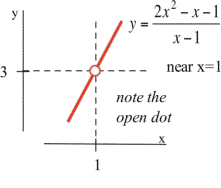
\includegraphics[width=0.4\textwidth]{img/chap2/image013.png}
    \label{$y=f(x)$ near $x=1$}
    \label{fig:2-4-limit-zoom}
\end{figure}
Notice that whenever $x$ is close to 1, the values of $y=f(x)$ are close to 3. Since $f$ is not defined at $x=1$, the graph has a hole above $x=1$, but we only care about what $f(x)$ is doing for $x$ close to but not equal to 1. Therefore,
$$\lim_{x\to 1}\dfrac{2x^2-x-1}{x-1}=\lim_{x\to 1}2x+1=3 \enspace.$$
\end{solution}\end{example}

\subsection{One Sided Limits}
Sometimes, what happens to us at a place depends on the direction we use to approach that place. If we approach Niagara Falls from the upstream side, then we will be 182 feet higher and have different worries than if we approach from the downstream side. Similarly, the values of a function near a point may depend on the direction we use to approach that point.

\definition[Left and Right Limits]
The {\bf left limit}\index{Limit!left} of $f(x)$ as $x$ approaches $c$ is $L$ if the values of $f(x)$ get as close to $L$ as we want when $x$ is very close to and left of $c$ (i.e., $x<c$). We write:
$$\lim_{x\to c^-}f(x)=L \enspace .$$
The{\bf right limit}\index{Limit!right} of $f(x)$ as $x$ approaches $c$ is $L$ if the values of $f(x)$ get as close to $L$ as we want when $x$ is very close to and right of $c$ (i.e., $x>c$). We write
$$\lim_{x\to c^+}f(x)=L \enspace .$$
\begin{example}
Evaluate the one sided limits of the function $f(x)$ graphed in Figure \ref{fig:2-4-fx-ex} at $x=0$ and $x=1$.

\begin{figure}[!ht]
  \centering
    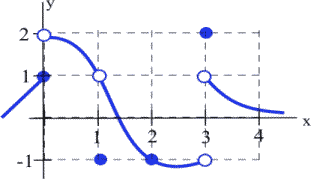
\includegraphics[width=0.4\textwidth]{img/chap2/image014.png}
    \caption{$y=f(x)$}
    \label{fig:2-4-fx-ex}
\end{figure}

\begin{solution} As $x$ approaches 0 from the left, the value of the function is getting closer to 1, so $\displaystyle\lim_{x\to 0^-}f(x)=1$.
As $x$ approaches 0 from the right, the value of the function is getting closer to 2, so $\displaystyle\lim_{x\to 0^+}f(x)=2$.
Notice that since the limit from the left and limit from the right are different, the general limit, $\displaystyle\lim_{x\to 0}f(x)$, does not exist.

At $x$ approaches 1 from either direction, the value of the function is approaching 1, so
$$\lim_{x\to 1^-}f(x)=\lim_{x\to 1^+}f(x)=\lim_{x\to 1}f(x)=1 \enspace.$$
\end{solution}\end{example}

\subsection{Continuity}
\label{ssec:continuity}
A function that is ``friendly'' and doesn't have any breaks or jumps in it is called {\bf continuous}\index{Continuous}. More formally,

\begin{definition}[Continuity at a Point]
A function $f(x)$ is {\bf continuous} at $x=a$ if and only if:
    \begin{enumerate}
    \item $f(a)$ exists,
    \item $\displaystyle\lim_{x\to a}f(x)$ exists, and 
    \item $\displaystyle\lim_{x\to a}f(x)=f(a)$.
    \end{enumerate}
\end{definition}
The graph in Figure \ref{fig:2-4-fx-continuity} illustrates some of the different ways a function can behave at and near a point, and the table contains some numerical information about the function and its behavior.
\begin{figure}[!ht]
  \centering
    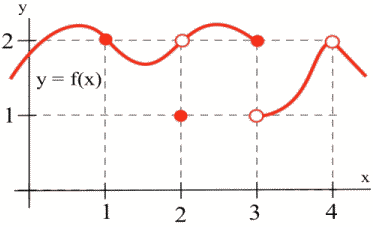
\includegraphics[width=0.4\textwidth]{img/chap2/image015.png}
    \caption{$y=f(x)$}
    \label{fig:2-4-fx-continuity}
\end{figure}

\begin{table}[ht!]
\begin{centering}
\begin{tabular}{ccc}
\toprule
$a$	& $f(a)$ &	$\displaystyle\lim_{x\to a}f(x)$ \\		
\midrule
1 &	2 & 2	\\
2 & 1 &	2\\
3 & 2 &	Does not exist (DNE)	\\
4 & Undefined &	2\\
\bottomrule
\end{tabular}
%\caption{}
%\label{tab:2-4-limitex2}
\end{centering}
\end{table}
	
Based on the information in the table, we can conclude that $f(x)$ is continuous at 1 since $\displaystyle\lim_{x\to 1}f(x)=2=f(1)$. We can also conclude from the information in the table that $f(x)$ is not continuous at 2, 3, or 4, because $\displaystyle\lim_{x\to 2}f(x)\neq f(2)$, $\displaystyle\lim_{x\to 3} f(x)\neq f(3)$, and $\displaystyle\lim_{x\to 4} f(x)\neq f(4)$.

The behaviors at $x=2$ and $x=4$ exhibit a hole in the graph, sometimes called a {\bf removable discontinuity}\index{Discontinuity!removeable}, since the graph could be made continuous by changing the value of a single point. The behavior at $x=3$ is called a {\bf jump discontinuity}\index{Discontinuity!jump} or {\bf step discontinuity}\index{Discontinuity!step}, since the graph jumps between two values. Jump discontinuities and vertial asymptotes are both {\bf nonremovable discontinuities}\index{Discontinuity!nonremoveable} because they cannot be fixed by changing the value of a single point.

So which functions are continuous? It turns out pretty much every function you've studied is continuous where it is defined: polynomial, radical, rational, exponential, and logarithmic functions are all continuous where they are defined. Moreover, any sum, difference, or product of continuous functions is also continuous.

This is helpful, because the definition of continuity says that for a continuous function, $\displaystyle\lim_{x\to a}f(x)=f(a)$. That means for a continuous function, we can find the limit by direct substitution (evaluating the function) if the function is continuous at $a$.

\begin{example}
Evaluate using continuity, if possible:
    \begin{enumerate}[label=(\alph*)]
    \item $\displaystyle\lim_{x\to 2}x^3-4x$

    \begin{solution} The given function is a polynomial, so it is defined for all values of $x$. Therefore, we can find the limit by direct substitution:
    $$\lim_{x\to 2}x^3-4x = 2^3-4(2) = 0 \enspace.$$
    \end{solution}
    \item $\displaystyle\lim_{x\to 2}\frac{x-4}{x+3}$

    \begin{solution} 
    The given function is rational. It is not defined at $x = -3$, but we are taking the limit as $x$ approaches 2, and the function is defined at that point, so we can use direct substitution:
    $$\lim_{x\to 2}\frac{x-4}{x+3} = \frac{2-4}{2+3}=-\frac{2}{5} \enspace .$$
    \end{solution}
    \item $\displaystyle\lim_{x\to 2} \frac{x-4}{x-2}$

    \begin{solution} 
    This function is not defined at $x = 2$, so is not continuous at $x = 2$. We cannot use direct substitution. There is also no factor of $x-2$ in the numerator, so the $x-2$ in the denominator cannot be canceled out to remove the discontinuity. Therefore, the limit does not exist.
    \end{solution}
\end{enumerate}

\subsection{Exercises}

\begin{enumerate}
    \item Use the graph to determine the following limits.
    \begin{figure}[!ht]
    \centering
    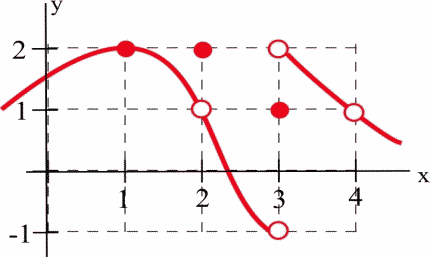
\includegraphics[width=0.4\textwidth]{img/chap2/image016.png}
    \end{figure}
    \begin{enumerate}[label=(\alph*)]
    \item $\displaystyle\lim_{x\to 1} f(x)$
    \item $\displaystyle\lim_{x\to 2} f(x)$
    \item $\displaystyle\lim_{x\to 3} f(x)$
    \item $\displaystyle\lim_{x\to 4} f(x)$
    \end{enumerate}

    \item	Use the graph to determine the following limits.
    \begin{figure}[!ht]
    \centering
    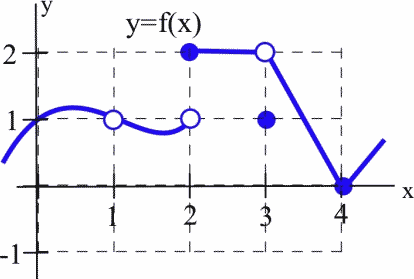
\includegraphics[width=0.4\textwidth]{img/chap2/image017.png}
    \end{figure}
    \begin{enumerate}[label=(\alph*)]
    \item $\displaystyle\lim_{x\to 1} f(x)$
    \item $\displaystyle\lim_{x\to 2} f(x)$
    \item $\displaystyle\lim_{x\to 3} f(x)$
    \item $\displaystyle\lim_{x\to 4} f(x)$
    \end{enumerate}


    \item	Evaluate the following. 
    \begin{enumerate}[label=(\alph*)]
    \item $\displaystyle\lim_{x\to 1}\dfrac{x^2 + 3x + 3}{x-2}$ 
    \item $\displaystyle\lim_{x\to 2}\dfrac{x^2 + 3x + 3}{x-2}$ 
    \end{enumerate}

    \item	Evaluate the following.
    \begin{enumerate}[label=(\alph*)]
    \item $\displaystyle\lim_{x\to 0}\dfrac{x + 7}{x^2+9x+14}$ 
    \item $\displaystyle\lim_{x\to 3}\dfrac{x + 7}{x^2+9x+14}$ 
    \item $\displaystyle\lim_{x\to -4}\dfrac{x + 7}{x^2+9x+14}$ 
    \item $\displaystyle\lim_{x\to -7}\dfrac{x + 7}{x^2+9x+14}$  
    \end{enumerate}


    \item At which points is the function shown discontinuous?

    \begin{figure}[!ht]
    \centering
    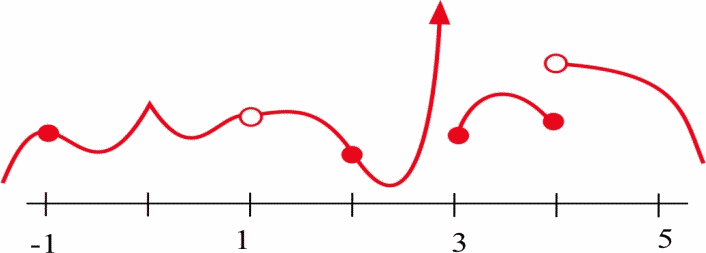
\includegraphics[width=0.4\textwidth]{img/chap2/image018.png}
    \end{figure}

    \item	At which points is the function shown  discontinuous?	

    \begin{figure}[!ht]
    \centering
    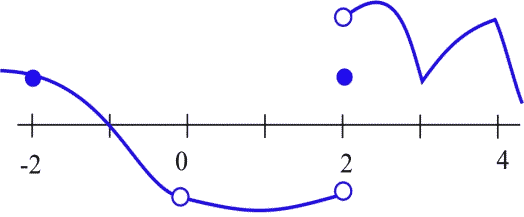
\includegraphics[width=0.4\textwidth]{img/chap2/image019.png}
    \end{figure}

    \item	Find at least one point at which each function is not continuous and  state which of the  three  conditions in the definition of continuity is 
	violated at that point.
    \begin{enumerate}[label=(\alph*)]
    \item $\dfrac{x-5}{x+3}$
    \item $\dfrac{x^2 + x -6}{x-2}$
    \item $\dfrac{x}{x}$
    \item $\dfrac{\pi}{x^2-6x+9}$
    \item $\ln(x^2)$
    \end{enumerate}
\end{enumerate}
\end{example}
